\cleardoublepage
\chapter*{Introduction}
\markboth{Introduction}{Introduction}
\addcontentsline{toc}{chapter}{Introduction}
% Here I bring the reader to general material science background to ML
% applications and their general importance, as well as the the study of
% representations as they are an essential building block

The discovery of new materials is one of the core pillars of technology, as
every technology relies on a material and, needless to say, would not exist
without it\cite{tomellini2013commentary}.
%[R. Tomellini, J. V. Benesch and A. Alming, Commentary: Fostering innovation
%in materials science and engineer].  A material can be more formally described
%by the configurations of atoms and the electron distribution.
The search for new materials is bound by thermodynamic laws which tell what
configurations are stable and can therefore be considered as potential
material.
%, i.e. can exist for a limited time frame under a certain set of thermodynamic
%boundary conditions.In the last decades it has been shown that \textit{ab initio} quantum chemistry
methods provide approximate stability criteria which are in good agreement with
experiments\cite{jansen2015conceptual} making them a viable tool for the
screening of new materials\cite{ceder1998identification, andersson2006toward,
yang2012search, gomez2016design}.  Due to the vast number of possible atomic
structures to be considered, the efficiency of these methods is crucial.

Data-driven methods have become an efficient extension reducing expensive
quantum chemistry calculations to a bare minimum while reaching
close-to-\textit{ab initio} accuracy over a wide configuration
space\cite{bartok2018machine}, leading to the exploration of previously
computationally intractable problems, such as the thermal conductivity of
amorphous germanium telluride\cite{sosso2012thermal}.  These methods are based
on transforming geometrical, physical and chemical information into a vector
representation, referred as descriptor, to then use it as features in a machine
learning model.  The development of expressive and computational inexpensive
descriptors\cite{behler2011atom, bartok2013representing} has lead to
applications in a wide range of areas\cite{mansouri2018machine,
sosso2018understanding, basdogan2019machine}.  Efficient descriptors are
therefore essential for state of the art high-throughput material design
application.

\begin{figure}
    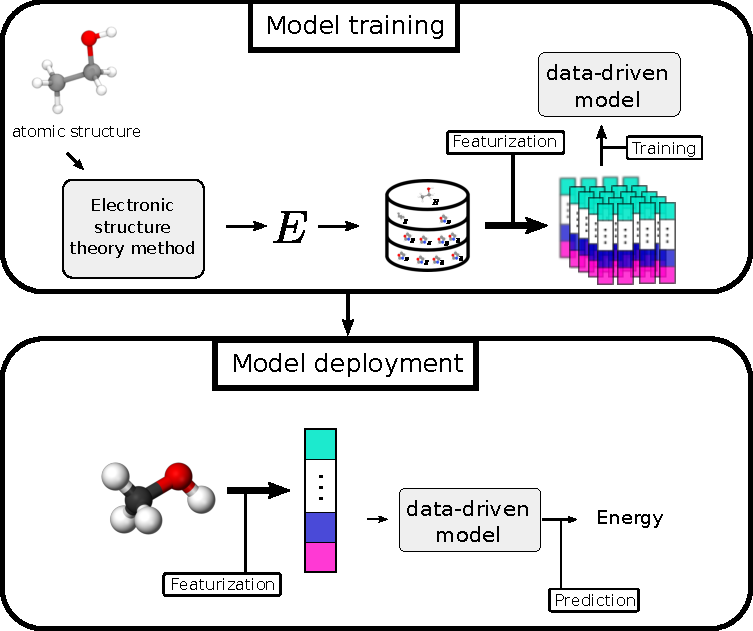
\includegraphics[width=\textwidth]{fig/slide5_0.pdf}
    \caption{A schematic showing the idea of high-throughput calculations with data-driven model that serves as surrogate model to bypass the expensive electronic structure theory calculations after a training the model.}
    \label{fig:high-throughput-scheme}
\end{figure}
%The key conceptual/domain part behind the methods determining their quality is
%the choice of description of the configuration called descriptor and the way
%to express similarity between these descriptions.

%0.5 page Statement of the problem and specific problem:
The efficient computation of expressive descriptors is a challenging problem which has seen a wide range of proposals\cite{behler2011atom, rupp2012fast, bartok2013representing, huo2017unified}.
%It has been shown that density-based state-of-the-art descriptors can be seen as different representations of the symmetrized many-body correlation function\cite{willatt2019atom}.
When used to build an interatomic potential, or to predict other atomic-scale properties, representations are used together with different supervised learning schemes, so it is difficult to disentangle the interplay of descriptor, regression method, and target property that combine to determine the accuracy and computational cost of the different methods.~\cite{zuo+20jpcl}
A deeper understanding of these descriptors is therefore essential, especially considering that the efficiency of accurate potentials is still a limiting factor for the research that can be conducted on materials.
%considering that blackbox machinaries as neural networks make it hard to specify what information contributed to their success making the improvement of models similar to try to hit a bin with a rock that lies in completely in the shadows.
%While neural networks have been successful in pushing the limits in inference accuray, due to their highly parametric nature they cannot compete with splining techniques.
%We have to take one step back and ask us do we really need this?

The first part of this thesis presents a collection of measures that serve as toolkit to guide the choice of the descriptor and model.
The second part discusses the implementation of machine learning model models as interatomic potentials, covering on one hand the efficient implementation of descriptors and data-driven models, and on the other hand their deployment into molecular dynamics software.

%The continuation of this development is the objective of this thesis.  The
%general goal of the thesis is the improvement of state of the art descriptors
%in terms of their encoded information and their concrete implementations.
%Since machine learning models are based on comparing features with the help of
%a similarity measurement, there is a strong connection between the similarity
%of two atomic configurations in form of their descriptor, and the Euclidean
%distance between their symmetrized many-body correlation function.
%The general goal of the thesis is the improvement of state of the art
%descriptors in terms of their encoded information and their concrete
%implementations.
%While the Euclidean distance can represent distances between close
%distributions accurately, more distant ones are not faithfully represented.
%On the other hand descriptors relying on sorting geometric
%information\cite{rupp2012fast, gallet2013structural} are similarly connected to
%the Wasserstein distance\cite{rowland2019orthogonal}.  The effect of the
%distance among atomic environments on the descriptor and subsequently on the
%regression of physical properties has not been extensively analyzed yet and is
%part of the objective of this thesis.  Such an analysis requires the
%development of measures for the comparison of feature spaces and efficient
%adaptations of the Wasserstein distance to a wider range of descriptors.

%Furthermore, recently generative models have been introduced for the generation
%of stable atomic configurations\cite{Sanchez-Lengeling360, gebauer2019symmetry,
%noe2019boltzmann, hoffmann2019data}.  The usage of descriptors in generative
%models requires a mapping of the descriptor back to the atomic configuration.
%Heretofore efficient inversion schemes have been introduced only for the
%3-dimensional atomic density function\cite{Sanchez-Lengeling360} and for
%distributions over distances between atoms\cite{gebauer2019symmetry}.  The
%development of an efficient inversion for state of the art descriptors which
%capture translational and rotational invariant many-body order information is
%an open problem which will be addressed with this thesis.
